\documentclass[12pt,a4paper]{scrartcl}

\usepackage[utf8]{inputenc}
\usepackage[T1]{fontenc}
\usepackage[british,UKenglish,USenglish,american]{babel}

\usepackage[pdftex]{graphicx}
\usepackage{latexsym}
\usepackage{amsmath,amssymb,amsthm}
\allowdisplaybreaks
\usepackage{dsfont}
\usepackage{pifont}
\usepackage{nicefrac}
\usepackage{textcomp}
\usepackage{enumitem}
\usepackage{lmodern}
\usepackage{bbm}

% Abstand obere Blattkante zur Kopfzeile ist 2.54cm - 15mm
\setlength{\topmargin}{-15mm}	   
                  
%\numberwithin{equation}{section} 
\numberwithin{equation}{subsection}

\newcommand{\C}{\mathbb{C}} % komplexe
\newcommand{\R}{\mathbb{R}} % reelle
\newcommand{\Q}{\mathbb{Q}} % rationale
\newcommand{\Z}{\mathbb{Z}} % ganze
\newcommand{\N}{\mathbb{N}} % natuerliche
\newcommand{\PP}{\mathbb{P}} % Probability
\newcommand{\E}{\mathcal{E}} % big Epsilon
\newcommand{\K}{\mathcal{K}}

\numberwithin{equation}{section}

\theoremstyle{definition}
\newtheorem{example}{Example}[subsection]
\newtheorem{theorem}{Theorem}[subsection]
\newtheorem{corollary}{Corollary}[subsection]
\newtheorem{lemma}{Lemma}[subsection]
\newtheorem{definition}{Definition}[subsection]
\newtheorem{proposition}{Proposition}[subsection]
\newtheorem{algorithm}{Algorithm}[subsection]
\newtheorem{prop}{Proposition}[subsection]
\newtheorem{remark}{Remark}[subsection]
\newtheorem{pro}{Proof}
\newtheorem{comment}{Comment}[subsection]


\begin{document}
	\pagestyle{empty}

\begin{titlepage}

	
\includegraphics[scale=0.45]{kit-logo.jpg} 
    \vspace*{2cm} 
\begin{center} \large 
    
   Masterthesis
    \vspace*{2cm}

    {\huge External DLA}\\
    \vspace*{2.5cm}

    Tillmann Tristan Bosch
    \vspace*{1.5cm}

    10. March 2020
    \vspace*{3.5cm}


    Supervisor: PD. Dr. Steffen Winter \\[1cm]
    Faculty of Mathematics\\[1cm]
	Karlsruhe Institute of Technology
\end{center}
\end{titlepage}

\newpage

\newpage
\phantom \\
\newpage

\tableofcontents %Inhaltsverzeichnis

 	\pagestyle{headings}

\setcounter{page}{1}


\newpage

\section{Introduction}
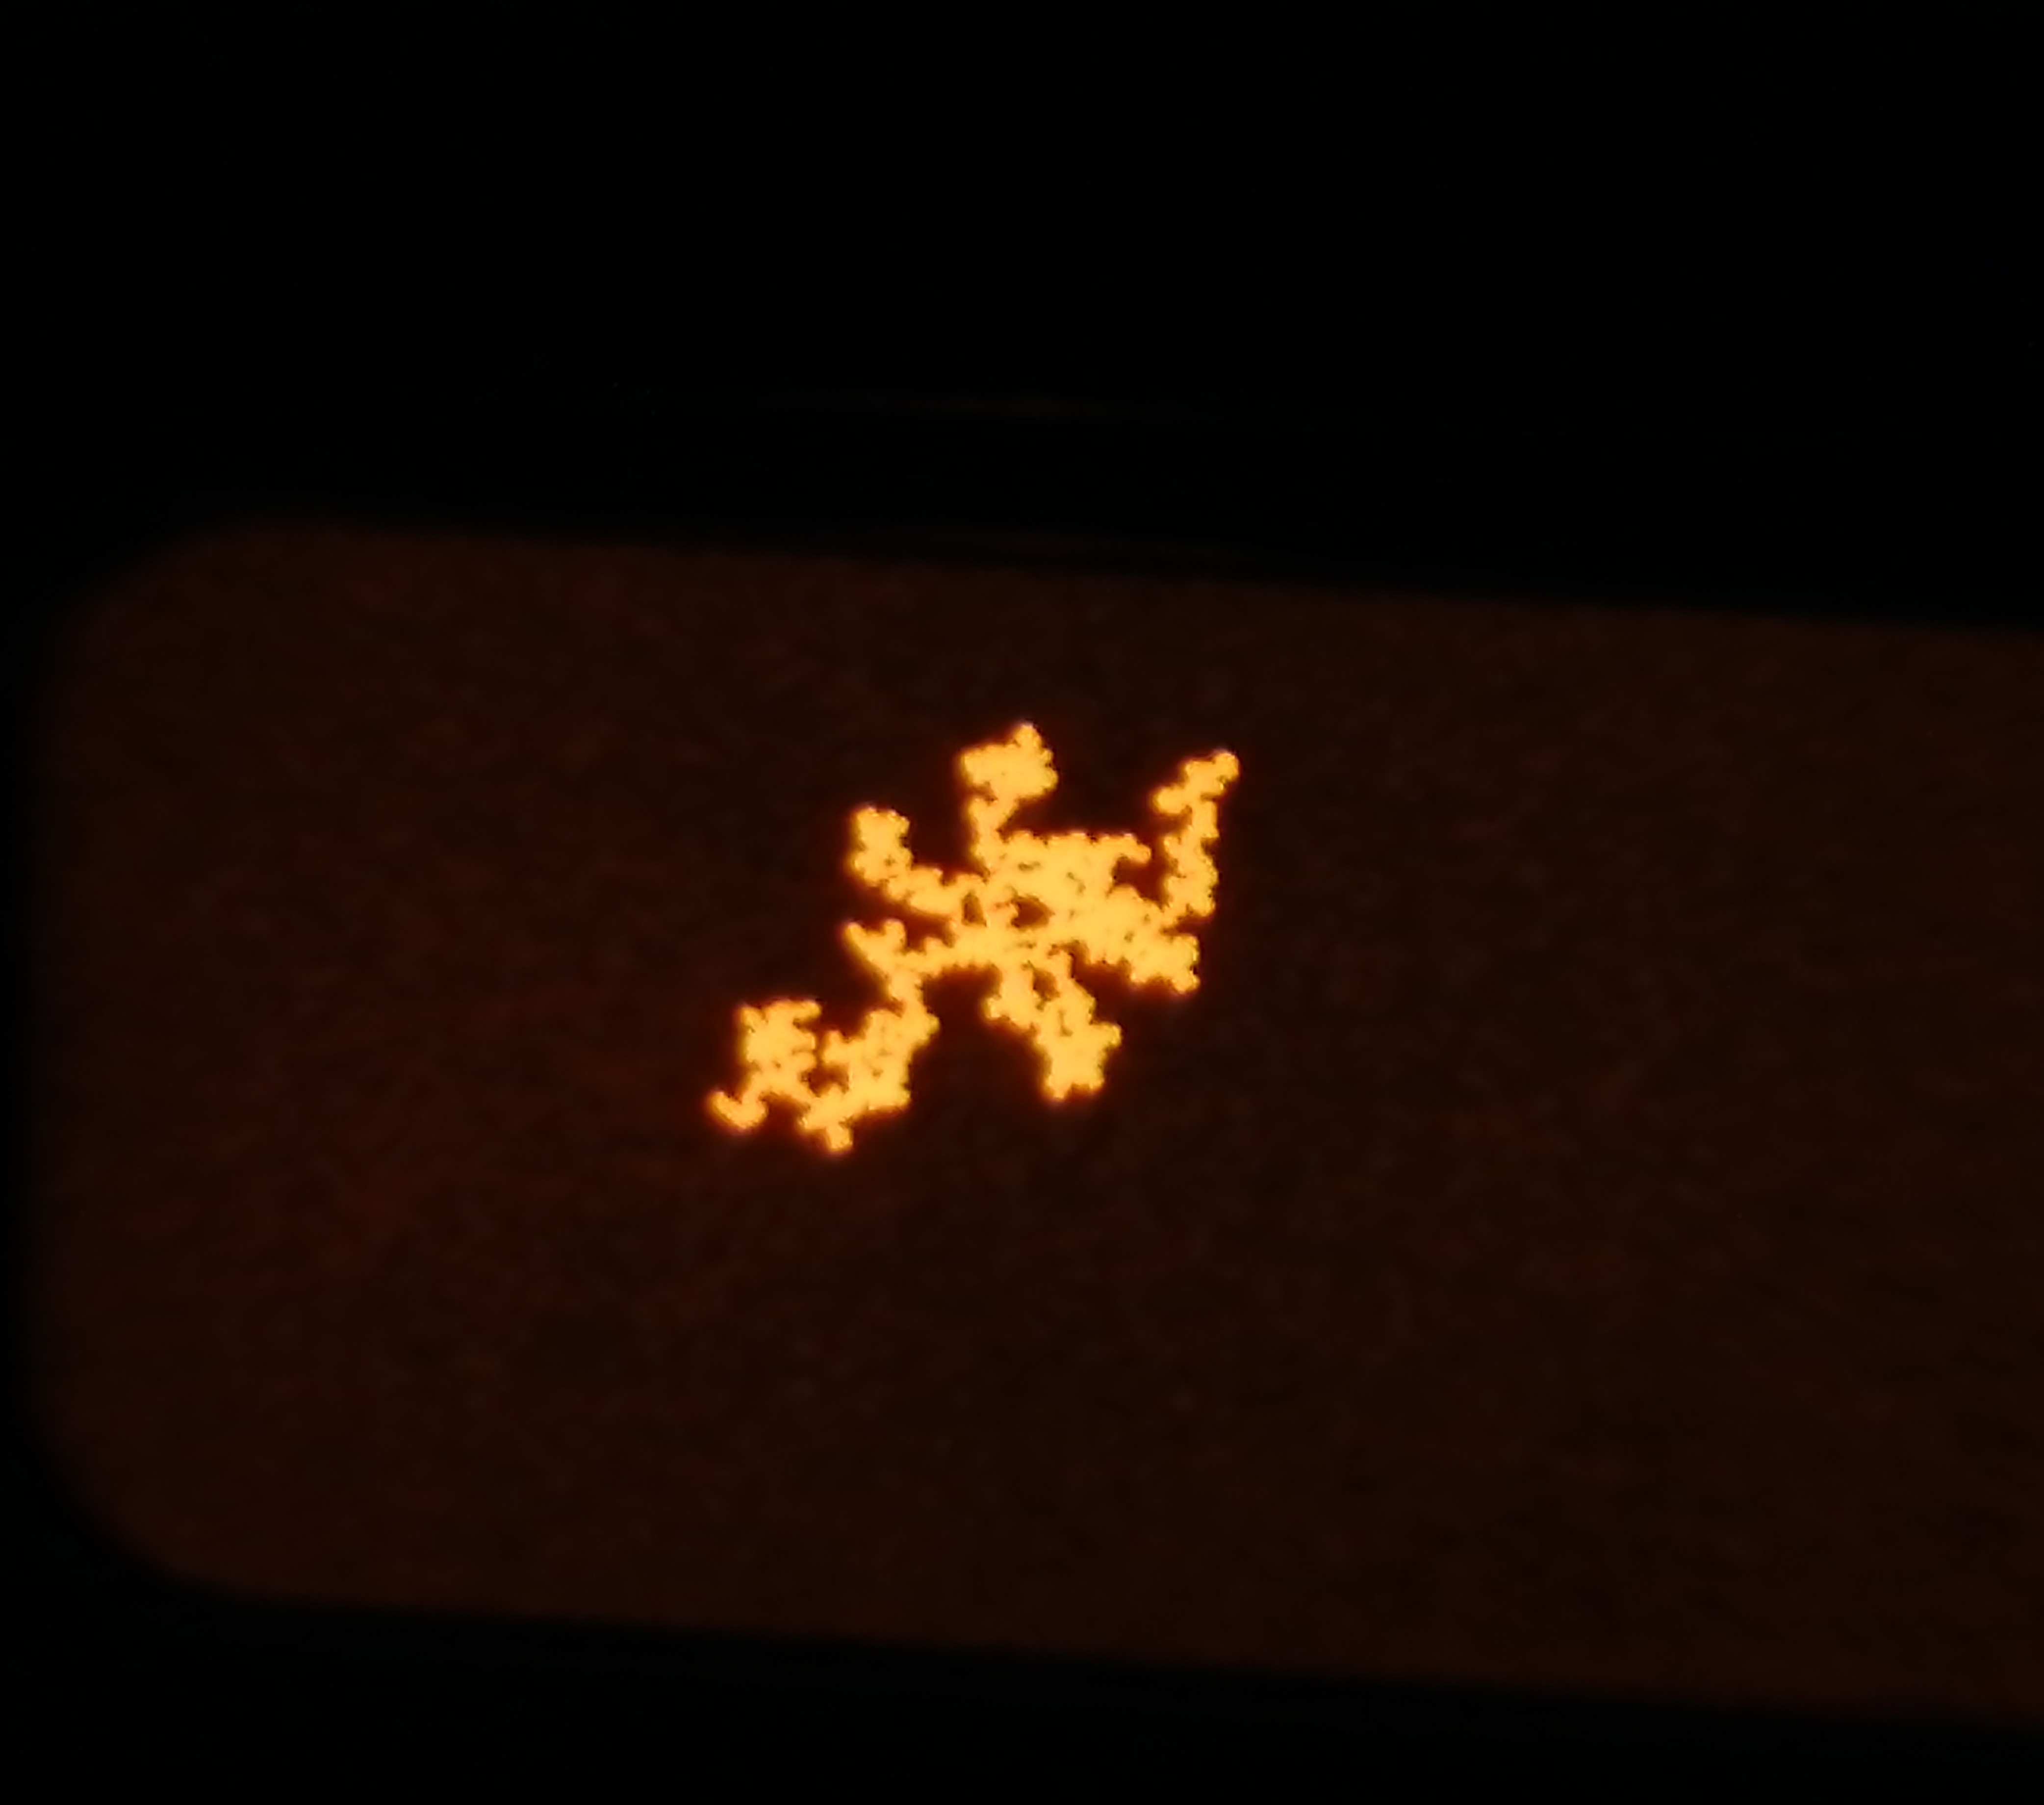
\includegraphics[scale=0.04]{display.jpg} 
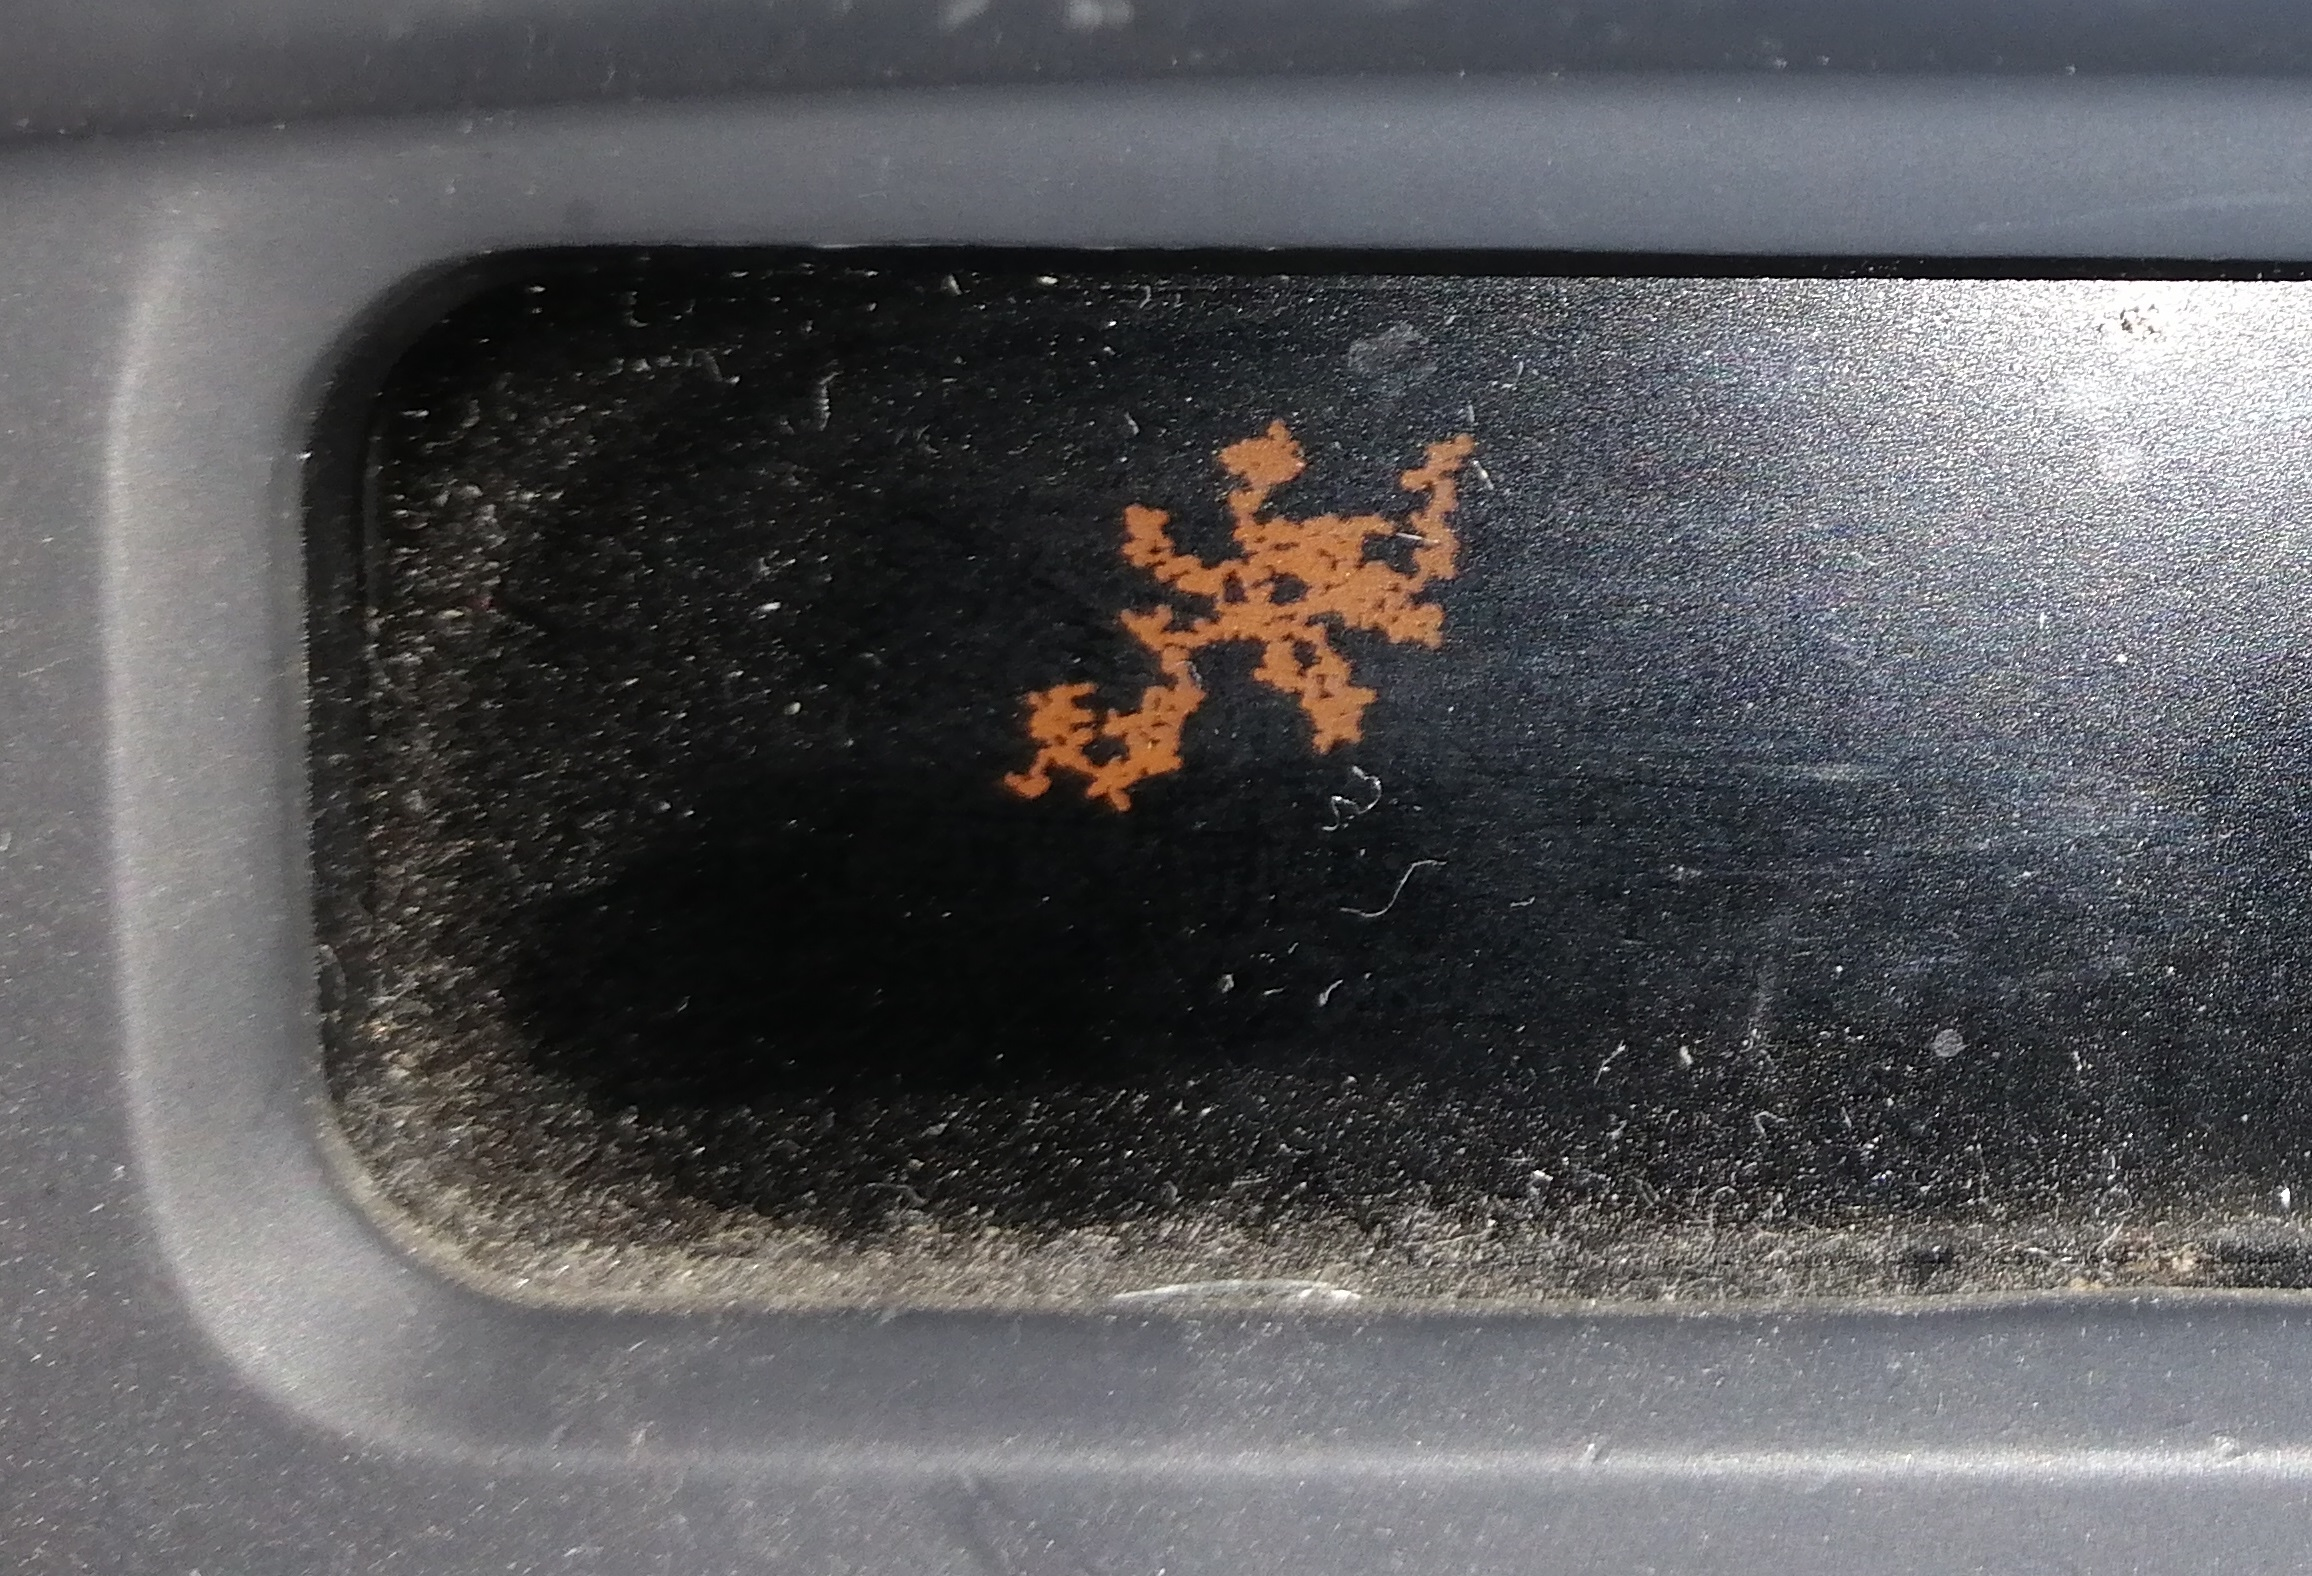
\includegraphics[scale=0.091]{display2.jpg}

\newpage


\section{Preliminaries} \label{prelim}

We prepare this script with the following preliminaries. \\
\\
\noindent $\boldsymbol{\mathit{General\ Definitions}}.\quad$ In this paper for practical purposes we will consider the natural numbers containing 0, so $\mathbb{N} := \{0, 1, 2, 3, \dots\}$. 
\\

\noindent $\boldsymbol{\mathit{Graphs}}.\quad$ We will be interested in the graph $(\mathbb{Z}^d, E)$ with its canonical graph structure, which is two vertices (or points) $x=(x_1,\dots,x_d),y=(y_1,\dots,y_d)\in \mathbb{Z}^d$ form an edge (e.q. $(x,y)\in E$) if and only if there exists exactly one $i\in \{1,\dots, d\}$ such that $|x_i - y_i| = 1$ and $x_j = y_j$ for all $j\neq i$. For a point $x\in \mathbb{Z}^d$ its set of $\mathit{neighbours}$ is defined as 
\begin{align*}
	N(x) := \{y\in \mathbb{Z}^d\ |\ (x,y)\in E\}
\end{align*}
and the canonical graph structure as defined above basically means that $N(x) = \{x+re_i\ |\ r\in \{-1,1\}\text{ and } i\in \{1,\dots, d\}\}$ where $e_i$ is the usual $i$-th standard basis vector of $\mathbb{Z}^d$, precisely $(e_i)_j=\delta_{ij}$ for all $i,j\in \{1, \dots , n \}$ where $\delta_{ij}=0$ if $i\neq j$ and $\delta_{ij}=1$ if $i=j$. For a set $A\subset \mathbb{Z}^d$ the $\mathit{outer\ boundary}\ \partial A$ of $A$ is defined as 
\begin{align*}
	\partial A := \{y\in \mathbb{Z}^d\setminus A\ |\ \exists x\in A:\ (x,y)\in E\}
\end{align*}
Instead of $(\mathbb{Z}^d, E)$ we will write $\mathbb{Z}^d$ from now on. 
\\

\noindent $\boldsymbol{\mathit{Probability\ Spaces}}.\quad$ Let $(\Omega,\mathcal{F}, \mathbb{P})$ be a probability space which we will base on in this paper. For our space of interest $\mathbb{Z}^d$ we will always use the discrete $\sigma$-Algebra which is the power set of $\mathbb{Z}^d$. If for $A\in \mathcal{F}$ we have $\mathbb{P}(A)=1$ we will say that $A$ holds $\mathbb{P}$-$a.s.$, or short $A$ holds $a.s.$ (almost sure).
\\

\noindent $\boldsymbol{\mathit{Random\ Walks}}.\quad$ First we define a $\mathit{Random\ Walk}$ on $\mathbb{Z}^d$ which we will use in this paper. A family $(S_n)_{n\in \mathbb{N}}$ of measurable functions $S_n: \Omega \to \mathbb{Z}^d$ is called a $\mathit{Random\ Walk\ on}\ \mathbb{Z}^d$ $\mathit{(starting\ at}\ x\in \mathbb{Z}^d)$ if and only if $S_0=x$ $a.s.$ and $\mathbb{P}(S_n\in N(y)\ |\ S_{n-1} = y) = 1$ for all $n \geq 1$ with 

\begin{align*}
	\mathbb{P}(S_n = y) = \frac{1}{|N(S_{n-1})|} = \frac{1}{2d}\quad \text{ for all }  y\in N(S_{n-1})\quad a.s., 
\end{align*}

note that $|N(y)| = 2d$ for all $y\in \mathbb{Z}^d$ since every point has two neighbours in every dimension. So a Random Walk can be understood as a particle starting from some point $x$ and moving randomly on the grid choosing its next step uniformly from its neighbour points. Furthermore define 

\begin{align*}
	\mathbb{P}_x(S_n\in A) := \mathbb{P}(S_n\in A|S_0=x)
\end{align*}

for any subset $A\subset G$. We define the $hitting\ time$ of A as 

\begin{align*}
	T(A) := \min \{n\geq 0\ |\ S_n\in A\},
\end{align*}

and $T(x):= T(\{x\})$ for one element sets and $x\in G$. The $heat\ kernel$ of the random walk $S_n$ is defined to be 

\begin{align*}
	p_n(x,y):=\mathbb{P}^n_x(S_n=y)
\end{align*}

and following the $\mathit{Green's\ function}$ as 

\begin{align*}
	G(x,y) := \sum_{n\geq 0} p_n(x,y).
\end{align*}

Similarily for a subset $A\subset G$ the $killed$ or $\mathit{stopped\ Green's\ function}$ is defined as

\begin{align*}
	G_A(x,y) := \sum_{n\geq 0} \mathbb{P}_x(S_n=y, T(A) > n).
\end{align*} 


\newpage
\section{Incremental Aggregate}
In this paper we will look at stochastic processes on the set of finite subsets of $\mathbb{Z}^d$, where we start with a one point set at $(0,0)$ and incrementally add a point on the outer boundary of the current cluster according to some distribution. What we get is a randomly, point-by-point growing connected cluster which here we will call $\mathit{Incremental\ Aggregate}$. Define 
\begin{align}
	\mathcal{P}_f := \{A\subset \mathbb{Z}^d\ |\ \text{A is finite}\}, 
\end{align}
the set of finite subsets of $\mathbb{Z}^d$. Furthermore we will be interested in distributions on those sets, so for $A\in \mathcal{P}_f$ we define 
\begin{align}
	\mathcal{D}_A:= \{\mu: \mathbb{Z}^d\to [0,1]\ |\ \mu(y) = 0 \text{ for all } y\notin A\ \text{and}\ \sum_{y\in A} \mu(y) = 1 \}.
\end{align}
So every element in $\mathcal{D}_A$ naturally defines a distribution on the elements of $A$. Now we define $\mathit{Incremental\ Aggregate}$ as follows.  

\begin{definition}
	Let $\mu=(\mu_A)_{A\in \mathcal{P}_f}$ be a family of distributions with $\mu_A\in \mathcal{D}_A$ for all $A\in \mathcal{P}_f$. $\mathit{Incremental\ Aggregate\ (with\ distribution\ \mu)}$ is a stochastic process $(\mathcal{E}_n)_{n\in{\mathbb{N}_0}}$ which evolves as follows. The process starts with one point $\mathcal{E}_0 = \{(0,0)\}$ in the origin of $\mathbb{Z}^d$. Knowing the process $\mathcal{E}_n$ at time $n$, let $y_n$ be a random point in $\partial \mathcal{E}_n\in \mathcal{P}_f$ with distribution
	\begin{align}
		\mathbb{P}(y_n = y\ |\ \mathcal{E}_n) := \mu_{\partial \mathcal{E}_n}(y),\quad y\in \mathbb{Z}^d.
	\end{align}
	We then define $\mathcal{E}_{n+1} := \mathcal{E}_n \cup \{y_n\}$.
\end{definition} 

\begin{remark}
	
\end{remark}



\newpage

\newpage
\section{External DLA}

External DLA is a model of Incremental Aggregate as defined above using a very natural distribution, called the $\mathit{harmonic\ measure}$. 

\begin{definition} $\mathit{(Harmonic\ Measure)}$\\
	\\
	Remembering the definitions in \eqref{prelim}, especially the heat kernel $p_n(x,y):=\mathbb{P}_x(S_n=y)$ of a random walk, the $\mathit{hitting\ distribution}$ of elements in $A$ with $\mathit{hitting\ position}$ $S_{T(A)}$ is 
	\begin{align*}
	H_A(x,y) := p_{T(A)}(x,y),\quad y\in A, 
	\end{align*}
	and for the special case $x=o:=(0,0)$ we define
	\begin{align*}
	h_A(y) := H_A(o,y) = \mathbb{P}_o(S_{T(A)}=y),\quad y\in A.
	\end{align*}
	Thus, $h_A(y)$ is the probability of hitting $A$ for the first time at $y$ starting from $o$. $h_A$ is called the $\mathit{harmonic\ measure\ (from\ o)}$.
\end{definition}

\begin{lemma}
	harmonic measure := hearmonic measure from infinity. Why does this exist?
\end{lemma}

\begin{definition} $\mathit{(External\ Diffusion\ Limited\ Aggregate,\ External\ DLA)}$\\
	\\ Incremental Aggregate with the harmonic measure $h$ as its distribution we define here, and in literature is known as $\mathit{Exernal\ Diffusion\ Limited\ Aggregate}$, short $\mathit{External\ DLA}$.
\end{definition}

\begin{remark}
	contenu...
\end{remark}

\newpage
\section{Integral Geometry}

In the next section we want to define an approximation for DLA. To do this we will need some concepts and results from Integral Geometry which we will discuss and develop in this section. Reminder: A set $K\subset \mathbb{R}^d$ is called $\mathit{convex}$ if and only if for any two points $a,b\in K$ we have that $\{ta + (1-t)b \in \mathbb{R}^d\ |\ t\in [0,1]\}\subset K$. The set of convex and compact subsets of $\R^d$ we call $\K^d$. 

\subsection{Intrinsic Volumes}

A useful concept to measure intrinsic geometrical properties of Borel-sets $K\subset \R^d$ are $\mathit{intrinsic\ volumes}$. We define the $d$-th intrinsic volume of $K$ as $V_d(K):=\lambda_d(K)$. Furthermore define $S_{d-1}(K)$ to be the $\mathit{surface\ area}$ of $V_d(K)$, which is formally defined as the Hausdorff-measure of $\partial K$. For the following theorem define 

\begin{flalign*}
	\kappa_d := V_d(B_d) \text{ for } d>0, \text{ and } \kappa_0:=1
\end{flalign*}

\noindent where we can calculate $V_d(B_d) = \frac{\pi ^{\frac{d}{2}}}{\Gamma(\frac{d}{2} + 1)}$ with the $\mathit{Gamma\ function}$ $\Gamma(x) := \int_0^\infty t^{x-1}e^{-t}dt,\ x>0$. 

\begin{lemma} \label{mink}
	If $K\subset \K^d$, then $S_{d-1}$ is equal to the $\mathit{outer\ Minkowski\ content}$, i.e.
	
	\begin{flalign*}
		S_{d-1}(K) = M_{d-1}(K) := \lim_{\varepsilon \searrow 0} \frac{1}{\varepsilon} (V_d(K_{\oplus \varepsilon}) - V_d(K)),
	\end{flalign*}
	
	where $K_{\oplus \varepsilon} = \{x\in \R^d\ |\ d(x,K)\leq \varepsilon\}$. It is easy to show, that $K_{\oplus \varepsilon} = K + \varepsilon B_d :=\{x+y\in \R^d\ |\ x\in K, y\in \varepsilon B_d\}$, where $B_d := \{x\in \R^d\ |\ d(0,x)\leq 1\}$.
\end{lemma}

\begin{proof}
	
\end{proof}


\begin{theorem} $(\mathit{Steiner\ Formula})$
	For $K\in \K^d$ there exist uniquely determined numbers $V_0(K),\dots, V_d(K)\in \R$, such that for each $\varepsilon\geq 0$ 
	\begin{flalign} \label{steiner}
		V_d(K+\varepsilon B_d) = \sum_{j=0}^{d} \kappa_{d-j} \varepsilon^{d-j} V_j(K). 
	\end{flalign}
	\begin{proof}
		\cite{stoch1} Theorem 3.32
	\end{proof}
\end{theorem}

\begin{definition}
	$V_0(K),\dots, V_d(K)$ are called $\mathit{intrinsic\ volumes}$ of $K$. 
\end{definition}

\begin{remark}\label{Vjprop}
	\begin{enumerate}[label=(\roman*)]
		\item What we get are functions $V_j:\K^d \to \R$ for the $j$-intrinsic volume $V_j$. It can be shown that every $V_j$ can be uniquely extended to a function $V_j: \mathcal{R}^d \to \R$, where $\mathcal{R}^d := \{\bigcup_{j=1}^n K_j\subset \R^d\ |\ n\in \N_0,K_j\in \K^d \}$ (\cite{stoch1} Theorem 4.10).
		\item The coefficients $\kappa_{d-j}$ are chosen such that the $V_j$ become independent of the dimension of the underlying space. This means that $V_j$ will assign the same value for $K$ if $K$ is considered to be subset of $\R^d$ or $\R^{\tilde{d}}$ for  $d<\tilde{d}$, although the unit balls $B_d$ and $B_{\tilde d}$ are different in those two spaces. This is why the $V_j$ are called $\mathit{intrinsic}$ volumes (REFERENCE). 
		\item For $\varepsilon = 0$ the right side of equation (\ref{steiner}) reduces to $V_d(K)$ which shows a consistency of the notation. 
		\item With Lemma (\ref{mink}) and equation (\ref{steiner}) we get $S_{d-1}(K) = \lim_{\varepsilon \searrow 0} \frac{1}{\varepsilon} (V_d(K + \varepsilon B_d) - V_d(K) = \kappa_1 V_{d-1}(K) = 2V_{d-1}(K)$, which will be a useful result. 
		\item It can be shown that $V_0(\emptyset)=\dots=V_d(\emptyset)=0$ and $V_0(K)=1$ if $K\neq \emptyset$ (REFERENCE). 
	\end{enumerate}
\end{remark}

\subsection{Random q-flats}

An interesting set in Integral Geometry is the set of $q$-dimensional affine subspaces in the $d$-dimensional real space, short $A(d,q)$ the set of $q$-flats in $\R^d$. 
Later we will be interested in choosing random lines in the real plane (i.e. $1$-flats in $\R^2$). For that we need a suitable $\sigma$-algebra and measure on $A(d,q)$ which we'll define now in this section. Let $G_d$ be the set of rigid motions (euclidean motions) in $\R^d$. For $r>0$ and $x\in \R^d$ define $B_d(r,x) := \{y\in \mathbb{R}^d\ |\ d(x,y) \leq r\}$ and $B_d:=B_d(1,0)$. 

\begin{definition}
	 For $r>0$ and $x\in \R^d$ define $A_d(r,x) := \{ F\in A(d,q)\ |\ F\cap B_d(r,x) \neq\emptyset \}$. Then the $\sigma$-algebra $\mathcal{A}(d,q)$ on $A(d,q)$ shall be defined by
	 \begin{flalign*}
	 	\mathcal{A}(d,q) := \sigma(\{ A_d(r,x)\ |\ r>0,x\in \R^d\}).
	 \end{flalign*} 
\end{definition}

\begin{theorem}
	On $A(d,q)$ there exists a unique $G_d$-invariant Radon measure $\mu_q$ such that
	\begin{flalign}
		\mu_q(A_d(1,0)) = \mu_q(\{F\in A(d,q)\ |\ F\cap B_d\neq \emptyset\}) = \kappa_{d-q}
	\end{flalign}
\end{theorem}
\begin{proof}
	\cite{stoch1} Theorem 4.26
\end{proof}

\begin{remark}
	$A_K\in \mathcal{A}(d,q)$ for $K\in\K^d$?
%	For a convex set $K\in \K^d$ since $K$ is closed we can write $K=(\bigcup_{j=0}^\infty B_d(r_j, x_j))^C$ for some $r_j>0$ and $x_j\in \R^d$. Then we get
%	\begin{flalign*}
%		A_K :&= \{F\in A(d,q)\ |\ F\cap K\neq \emptyset\} 
%		\\ &= \{F\in A(d,q)\ |\ F\cap (\bigcup_{j=0}^\infty B_d(r_j, x_j))^C \neq \emptyset\} 
%		\\ &= \{F\in A(d,q)\ |\ F\cap \bigcap_{j=0}^\infty B_d(r_j, x_j)^C \neq \emptyset\} 
%		\\ &= \{F\in A(d,q)\ |\ \bigcap_{j=0}^\infty F\cap B_d(r_j, x_j)^C\neq \emptyset\}
%		\\ &= \{F\in A(d,q)\ |\ F\cap B_d(r_j, x_j)^C\neq \emptyset\text{ for all } j>0 \}
%		\\ &\supset \{F\in A(d,q)\ |\ F\cap B_d(r_j, x_j) = \emptyset\text{ for all } j>0 \}
%		\\ &= \bigcap_{j=0}^\infty \{F\in A(d,q)\ |\ F\cap B_d(r_j, x_j)= \emptyset\}
%		\\ &= \bigcap_{j=0}^\infty A_d(r_j, x_j)^C
%		\\ &= (\bigcup_{j=0}^\infty A_d(r_j, x_j))^C.
%	\end{flalign*}
\end{remark}

\begin{theorem} $(\mathit{Crofton\ formula})$
	Let $K\in \K',k\in \{1,\dots,d-1\}$ and $j\in \{ 0,\dots,k\}$. Then
	\begin{flalign}
		\int_{A(d,k)} V_j(K\cap F) \mu_k(dF) = c^{k,d-k+j}_{j,d}V_{d-k+j}(K),
	\end{flalign} 
	where $c_s^r := \frac{r!\kappa_r}{s!\kappa_s}$ for $s,r\in \N_0$ and $c^{r_1,\dots,r_k}_{s_1,\dots,s_k} := \prod_{j=1}^k c_{s_j}^{r_j}$. 
\end{theorem}

\begin{proof}
	\cite{stoch1} Theorem 4.27
\end{proof}

\begin{definition}
	Let $K_0\in \K^d$ with $V_d(K_0)>0$. Let $q\in \{0,\dots,d-1\}$. A $A(d,q)$-valued random element $X_q$ with distribution $\frac{\mu_q(\ \cdot\ \cap\ A_{K_0})}{\mu_q(A_{K_0})}$ is called an $\mathit{isotropic\ random\ q}$-$\mathit{flat}$ through $K_0$. 
\end{definition}

\begin{lemma} \label{K}
	Let $K,K_0\in \K^d$ with $K\subset K_0$ and $V_d(K_0)>0$. Let $q\in \{0,\dots,d-1\}$ and $X_q$ be an isotropic random $q$-flat through $K_0$. Then
\begin{flalign}
	\PP(X_q\cap K\neq \emptyset) = \frac{V_{d-q}(K)}{V_{d-q}(K_0)}. 
\end{flalign}
\end{lemma}
\begin{proof}
	We directly get
	\begin{flalign*}
		\PP(X_q\cap K \neq \emptyset) &= \PP(X_q\in A_K)
		= \frac{\mu_q(A_K\cap A_{K_0})}{\mu_q(A_{K_0})}
		\\ &= \frac{\mu_q(A_K)}{\mu_q(A_{K_0})}
		= \frac{\int_{A(d,q)} \mathbbm{1}\{F\cap K\neq \emptyset\} \mu_q(dF)}{\int_{A(d,q)} \mathbbm{1}\{F\cap K_0\neq \emptyset\} \mu_q(dF)}
		\\ &= \frac{\int_{A(d,q)} V_0(F\cap K) \mu_q(dF)}{\int_{A(d,q)} V_0(F\cap K_0) \mu_q(dF)}
		 \overset{Crofton}{=} \frac{c^{q,d-q}_{0,d}V_{d-q}(K)}{c^{q,d-q}_{0,d}V_{d-q}(K_0)}
		\\ &= \frac{V_{d-q}(K)}{V_{d-q}(K_0)}.
	\end{flalign*}
\end{proof}

\begin{remark} \label{S=2V}
	Taking the situation from the last Lemma, with Remark (\ref{Vjprop}) (iv) and $q=1$ we get
	\begin{flalign*}
		\PP(X_1\cap K \neq \emptyset) = \frac{V_{d-1}(K)}{V_{d-1}(K_0)} = \frac{S_{d-1}(K)}{S_{d-1}(K_0)}. 
	\end{flalign*}
	For $d=2$ we basically can interpretate, that the propability of a line $X_1$ which intersects $K_0$ also interesects $K$ can be calculated by deviding the boundary length of $K$ by the boundary length of $K_0$. This seems to be a convenient result although it may not be completely intuitive. 
\end{remark}





\subsection{Constructions in the real plane}

From now on consider the case $d=2$ and $q=1$ which is looking at lines in the real plane. For some $K_0\in \K^2$ we will be interested in choosing a random line which intersects with $K_0$. We have looked at exactly this situation in Lemma (\ref{K}). We will look at some examples in this section, argue about why the measure $\mu_1$ is senseful to be used and what parametrisations on lines could be helpful to actually calculate realisations for random lines equivalently to $\mu_1$. In the next chapter we'll define an Incremental Aggregate where we'll use our insights here to realise random lines. Note that every line $X\in A:=A(2,1)$ has a form $X=X_{a,b}:=\{a+tb\in \R^2\ |\ t\in \R^2\}$ for some vectors $a,b\in \R^2$ with $b\neq (0,0)$. From now on for $r>0$ and $x\in \R^2$ define $B_r(x):= \{y\in R^2\ |\ d(x,y)\leq r\}$ and $B_r:=B_r(0)$. Let furthermore $X_1$ be an isotropic random $1$-flat through $K_0$. Recap the definition of $\kappa_j$, which is the $j$-dimensional Lebesgue measure of the $j$-dimensional unit ball, for our use here $\kappa_0=1$, $\kappa_1 = 2$ and $\kappa_2 = \pi$. For the next examples we always use Lemma (\ref{K}) and Remark (\ref{S=2V}) (iii) and choose $K,K_0\in \K^2$ with $K\subset K_0$. 

\begin{example}
	Let $0<r<R$, $K_0 := B_R$ and $K:=B_r$. We get
	\begin{flalign*}
		\PP(X_1\cap B_r\neq\emptyset) = \frac{V_1(B_r)}{V_1(B_R)} = \frac{\frac{1}{2}S_1(B_r)}{\frac{1}{2}S_1(B_R)} = \frac{2\pi r}{2\pi R} = \frac{r}{R}. 
	\end{flalign*}
\end{example}

\begin{example}
	Let $0<r\leq \frac{R}{\sqrt{2}}$, $K_0 := B_R$ and $K:= [-r,r]^2$. We get 
	\begin{flalign*}
		\PP(X_1\cap [-r,r]^2 \neq\emptyset) = \frac{S_1([-r,r]^2)}{S_1(B_R)} = \frac{8r}{2\pi R} = \frac{4}{\pi} \frac{r}{R}. 
	\end{flalign*}
\end{example}

\begin{example}
	Let $0<r\leq R$, $K_0 := B_R$ and $K:=[-r,r]$. We get 
	\begin{flalign*}
	\PP(X_1\cap [-r,r] \neq\emptyset) = \frac{V_1([-r,r])}{V_1(B_R)} = \frac{\lambda_1([-r,r])}{\frac{1}{2}S_1(B_R)} = \frac{2r}{\pi R} = \frac{2}{\pi} \frac{r}{R}. 
	\end{flalign*}
\end{example}

\begin{example}
	Let $K_0 := B_1$ and $K:=T_a$ a equilateral triangle with side length $a=\frac{\pi}{3}$ centered at $(0,0)$. We get 
	\begin{flalign*}
	\PP(X_1\cap T_a\neq\emptyset) = \frac{V_1(T_a)}{V_1(B_1)} = \frac{3a}{2\pi} = \frac{1}{2}.
	\end{flalign*}
\end{example}



\begin{remark}
	We still haven't answered why $\mu_1$ is a senseful measure to be used to calculate probabilities for situations like in the last examples. And yet it is not obvious how to actually simulate a realisation of a random line with $\mu_1$. For now we can calculate the probability that a random line $X_1$ hits some convex set $K$ in the base set $K_0$. What we need is some form of parametrisation of this random choosing so we can actually end up for example with one angle defining the rotation of $X_1$ to the $x$-axis and a real number defining the interesection value of $X_1$ with the $y$-axis. If we wouldn't know about $\mu_1$ for now, we could choose an angle and a real number intuitively the following way: Choose an angle $\alpha$ uniformly out of $[0,\pi)$. Then consider all lines in the plane which are rotated counterclockwise by $\alpha$ starting at the $x$-axis and which intersect $K$. Take the set of intersection values of these lines with the $y$-axis and choose a value $y_0$ uniformly out of it, so finally $\alpha$ and $y_0$ define a unique line and we have a realisation of a random line which interesects $K$. This procedure may sound balanced, but it is only if $K_0$ is strongly symmetric. At this point it is important to remember what exactly we want. Out of all lines which intersect $K_0$ we are looking for the probability that a random chosen line intersects $K$ and finally calculate a realisation. Imagine $K_0=[-a,a]\times [-b,b]$ with $a<b$. Then it makes sense that there are "more" lines through the longer side $[-b,b]$ than through the shorter side $[-a,a]$. If we now choose the angle $\alpha$ uniformly, the shorter side is overweighted and the larger side underweighted, or in other words, the angle area around $\frac{\pi}{2}$ should be more likely to be chosen than the angle area around $0$. So this naive attempt of choosing the angle for our line uniformly doesn't consider asymmetries of $K_0$ and does therefore not hold the senseful idea, that longer sides of $K_0$ are hit by more lines than shorter ones. 
\end{remark}


\newpage

\section{Line Hitting Aggregate}

In the following we will look at a process which is the approach of a simple approximation of external DLA on $\mathbb{Z}^2$. The idea is to let particles move on straight lines coming from infinity and add to the cluster when hitting it. Obviously in most cases particles cannot move completely straight on $\mathbb{Z}^2$. Therefore we will consider points in $\mathbb{Z}^2$ as the centers of unit squares and let the particles move on straight lines in the full plane $\mathbb{R}^2$. We consider a line hitting a point in $\mathbb{Z}^2$ if and only if it intersects with its unit square as defined in the following. 

\begin{definition}
	Define 
	\begin{align}
		\mathbb{R}^2_{sq} := \{[k - \frac{1}{2}, k + \frac{1}{2}] \times [l- \frac{1}{2}, l + \frac{1}{2}] \subset \mathbb{R}^2\ |\ k,l \in \mathbb{Z}\}, 
	\end{align} 
	note that $\mathbb{R}^2 = \bigcup_{s\in \mathbb{R}^2_{sq}} s$. The canonical function
	\begin{align}
	sq: \mathbb{Z}^2 \to \mathbb{R}^2_{sq},\quad (k,l)\to [k - \frac{1}{2}, k + \frac{1}{2}] \times [l- \frac{1}{2}, l + \frac{1}{2}]
	\end{align}
	is bijective and intuitively identifies points in $\mathbb{Z}^2$ with squares in $\mathbb{R}^2$, which is $p$ is the center of square $sq(p)$ for all $p\in \mathbb{Z}^2$. In the following when using a point $p\in \mathbb{Z}^2$ it will reference the point in $\mathbb{Z}^2$ or the corresponding square in $\mathbb{R}^2$ respecting the context. This bijection also naturally defines a graph structure on $\mathbb{R}^2_{sq}$, which is two squares $s_1, s_2\in \mathbb{R}^2_{sq}$ form an edge if and only if $sq^{-1}(s_1)$ and $sq^{-1}(s_2)$ form an edge in $\mathbb{Z}^2$. 
	\noindent For the following context we say a line $L$ $hits$ a point $p\in \mathbb{Z}^2$ if and only if $L\ \cap\ sq(p) \neq \emptyset$.
	
\end{definition}

BILD Linie durch squares "hitting"\\


\begin{definition}
	Geradenmaß $\mu_0$
\end{definition}


\begin{definition}
	Let $L=L_{a,b}\in \mathcal{L}$ be a line. For a finite set $A\in \mathcal{P}_f$ we define 
	
	\begin{align*}
		L_{A} := \{ p\in A\ |\ L \text{ hits } p\}
	\end{align*}
	
	which is the subset of points in $A$ are hit by the line $L$ hits. For the following we suppose $L_A \neq \emptyset$. We want to define a total ordered relation $<_{line}$ on $L_A$. We choose two points $(x_1,x_2),(y_1,y_2)\in L_A$ and devide the definition of a relation into four cases, which are the line going from left-bottom to right-top, left-top to right-bottom, parallel to the $x$-axis and parallel to the $y$-axis. Write $b=(b_1,b_2)$.  \\
	\\
	$\mathit{Case\ 1:}\quad L\ \text{ is parallel to the x-axis}\quad \Leftrightarrow\quad b_2=0$
	\begin{align*}
	(x_1, x_2) <_{line} (y_1, y_2) \quad :\Leftrightarrow \quad x_1 < y_1
	\end{align*}\\
	$\mathit{Case\ 2:}\quad L\ \text{ is parallel to the y-axis}\quad \Leftrightarrow\quad b_1=0$
	\begin{align*}
	(x_1, x_2) <_{line} (y_1, y_2) \quad :\Leftrightarrow \quad x_2 < y_2
	\end{align*}\\
	$\mathit{Case\ 3:}\quad L\ \text{ is going from left-bottom to right-top}\quad \Leftrightarrow\quad b_1b_2>0$
	\begin{align*}
	(x_1, x_2) <_{line} (y_1, y_2) \quad :\Leftrightarrow \quad
		\begin{cases}
			x_1 < y_1, & \text{ if } x_1 \neq y_1, \\
			x_2 < y_2, & \text{ if } x_1 = y_1.
		\end{cases}
	\end{align*}\\
	$\mathit{Case\ 4:}\quad L\ \text{ is going from left-top to right-bottom}\quad \Leftrightarrow\quad b_1b_2<0$
	\begin{align*}
	(x_1, x_2) <_{line} (y_1, y_2) \quad :\Leftrightarrow \quad
	\begin{cases}
	x_1 < y_1, & \text{ if } x_1 \neq y_1, \\
	x_2 > y_2, & \text{ if } x_1 = y_1.
	\end{cases}
	\end{align*}\\
	It is easy to see that this well-defines a relation on $L_A$. In the following we will quickly proove that this relation is totally ordered. 
\end{definition}

\begin{lemma}
For a line $L=L_{a,b}\in \mathcal{L}$ and $A\in \mathcal{P}_f$ with $L_A\neq \emptyset$ the relation $<_{line}$ on $L_A$ is totally ordered. 
	\begin{proof}
		We will only proove the case where $L$ is going from left-bottom to right-top, which is $\mathit{Case\ 3}$ of the definition. In this case we have $b_1b_2>0$. Note, that the proof for $\mathit{Case\ 4}$ will work very similair. And in the case of $L$ being parallel to one of the axes ($\mathit{Case\ 1\ or\ 2}$), all properties for a totally ordered relation follow directly from the totally ordered relation $<$ on $\mathbb{R}$. So let $b_1b_2>0$. \\
		\\
		$\mathit{Antisymmetry:}$ For antisymmetry let $(x_1, x_2) <_{line} (y_1, y_2)$ and $(y_1, y_2) <_{line} (x_1, x_2)$. Suppose $x_1\neq y_1$, then $x_1 < y_1$ and $y_1 < x_1$, therefore $x_1 = y_1$ by antisymmetry of the standard order $<$ in $\mathbb{R}$, a contradiction, hence $x_1 = y_1$. But then we have $x_2 < y_2$ and $y_2 < x_2$ and therefore also $x_2 = y_2$. \\
		\\
		$\mathit{Transitivity:}$ For transitivity let $(x_1,x_2) <_{line} (y_1,y_2)$ and $(y_1,y_2) <_{line} (z_1,z_2)$. We find four cases. In case $x_1 \neq y_1$ and $y_1 \neq z_1$ we get $x_1 < z_1$ by transitivity of $<$, hence $(x_1,x_2) <_{line} (z_1,z_2)$. In case $x_1\neq y_1$ and $y_1 = z_1$ we get $x_1 < y_1 = z_1$, therefore $(x_1,x_2) <_{line} (z_1,z_2)$. In case $x_1 = y_1$ and $y_1 \neq z_1$ we get $x_1 = y_1 < z_1$, similair as the last case. In the last case $x_1 = y_1 = z_1$ we get $x_2 < y_2$ and $y_2 < z_2$ and again by transitivity of $<$ we get $x_2 < z_2$, hence $(x_1,x_2) <_{line} (z_1,z_2)$ again. \\
		\\
		$\mathit{Connexity:}$ Connexity is given since for any two points $(x_1,x_2),(y_1,y_2)\in L_A$ we have either $x_1 \neq y_1$ or $x_1 = y_1$ and therefore either $(x_1,x_2)<_{line}(y_1,y_2)$ or $(y_1,y_2)<_{line}(x_1,x_2)$.
	 
	\end{proof}
\end{lemma}

\begin{remark}
	The relation $<_{line}$ on $L_A$ basically orders the hitpoints of a line $L$ with a finite set $A$ from left to right (or bottom to top in case of a line parallel to the $y$-axis). This order allows us to identify the outest hitting points of $A$ by $L$. This means when moving on a line $L$ facing $A$ this order allows us to know where in $A$ the line $L$ hits first when ,,entering`` $A$ and where it hits last when ,,leaving`` $A$ which will be the two points $min_{<_{line}}L_A$ and $max_{<_{line}}L_A$ (or the other way around). 
\end{remark}


\begin{definition} $\mathit{Random\ Line\ Hitting\ Distribution}$\\
	\indent Choose $A\in \mathcal{P}_f$. We define a distribution $\mu_A$ on $\mathbb{Z}^2$ as in the following. 
	Let $L=L_{a,b}$ be a random line according to the line measure $\mu_0$ with the condition that $L$ hits $A$. Then define $\mu_A$ with distribution $\mu_A \sim U(\{min_{<_{line}}L_A, max_{<_{line}}L_A\})$, which chooses uniformly an element out of $\{min_{<_{line}}L_A, max_{<_{line}}L_A\}$. We call this distribution the $\mathit{Random\ Line\ Hitting\ Distribution\ (of\ A)}$.
\end{definition}

\begin{definition} $\mathit{Line\ Hitting\ Aggregate}$\\
	\indent Incremental Aggregate with the Random Line Hitting Distribution as its distribution we will call here $\mathit{Line\ Hitting\ Aggregate}$, short $\mathit{LHA}$. 
\end{definition}

\newpage
\section{Questions}
$\mathcal{K}'=?$

\newpage

\begin{thebibliography}{biblio}
\thispagestyle{empty}

\bibitem{Henze Skript}
N. Henze.
\emph{Maß und Wahrscheinlichkeitstheorie (Stochastik II)}.
Karlsruher Institut für Technologie, Karlsruhe, 2010

\bibitem{stoch1}
Daniel Hug, Günter Last, Steffen Winter.
\emph{Stochastic Geometry, 	Lecture Notes (summer term 2020)}.
Institute of Technology, Karlsruhe



\end{thebibliography}

\newpage
  
\thispagestyle{empty}

\vspace*{8cm}


\section*{Erklärung}

Hiermit versichere ich, dass ich diese Arbeit selbständig verfasst und keine anderen als die angegebenen Quellen und Hilfsmittel benutzt, die wörtlich oder inhaltlich übernommenen Stellen als solche kenntlich gemacht und die Satzung des Karlsruher Instituts für Technologie zur Sicherung guter wissenschaftlicher Praxis in der jeweils gültigen Fassung beachtet habe. \\[2ex] 

\noindent
Karlsruhe, den 10. März 2020\\[5ex] 

\end{document}

